\documentclass{beamer}

\begin{document}
	
	\begin{frame}
	\frametitle{Hue: BGR}
		\begin{itemize}
			\item The (\colorbox{blue}{B},\colorbox{green}{G},\colorbox{red}{R}) color space can be visualized into the following coordinate system which is not very intuitive:
			
			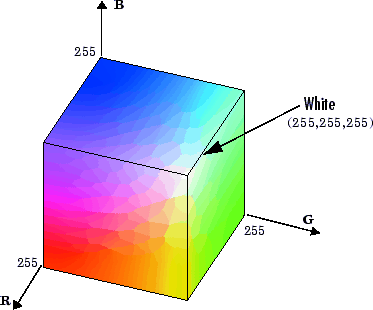
\includegraphics[scale = 0.7]{RGBcube}
			
			\pause
			
			\item A more intuitive way of representing the color is needed.
		\end{itemize}
	\end{frame}
	
	\begin{frame}
	\frametitle{Hue: Hue Saturation and Value}
		\begin{itemize}
			\item Luckily, the \colorbox{blue}{B}\colorbox{green}{G}\colorbox{red}{R} cube can be transformed into something more intuitive. That is the HSV cone:
			
			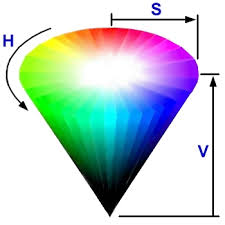
\includegraphics[scale = 0.6]{HSVcone}
			
			\pause
			
			\item By tilting the \colorbox{blue}{B}\colorbox{green}{G}\colorbox{red}{R} cube and letting it stand on its origin, you can obtain this HSV cone.
		\end{itemize}
	\end{frame}
	
	\begin{frame}
	\frametitle{Hue: A Polar Coordinate Representation of BGR cube}
		
		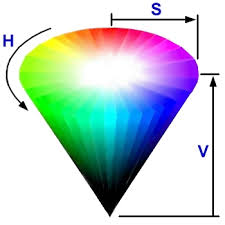
\includegraphics[scale = 0.4]{HSVcone}
	
		\begin{itemize}
			
			\item Analogous to how Cartesian coordinate gets transformed into polar coordinate, the transformation of \colorbox{blue}{B}\colorbox{green}{G}\colorbox{red}{R} cube into HSV cone is similar.
			
			\pause
			
			\item However, the purpose of this transformation is to get rid of unnecessary information contained in the \colorbox{blue}{B}\colorbox{green}{G}\colorbox{red}{R} color space.
			
			\item Since the saturation in HSV color space only denotes the degree of shade (or darkness) in the color, and the value in HSV only denotes its tint (or whiteness), only the hue in HSV gets to control the color as we see it!
		\end{itemize}
	\end{frame}
	
	\begin{frame}
	\frametitle{Hue: The Metric}
		
		\begin{itemize}
			\item What we did, then, is we extracted only the hue values out of our image matrix. In other words we hashed the matrix for an easier comparison.
			
			\item And the idea for this metric is that if two matrices are of the similar hue, there might not be a scene change. Vice versa.
		\end{itemize}
	\end{frame}
	
\end{document}